
\section{Analytical workflows}\label{analytical-workflows}


\subsection{Overview}\label{overview}

Table \ref{tab:tab-wflow} presents an informal topical
labeling for Bioconductor software packages with
cancer mentioned in the Description field of package
metadata.

\begin{table}
\caption{\label{tab:tab-wflow}Topical organization of packages with cancer applications.}
\begin{tabular}{lp{6cm}}
\toprule
topic & packages\\
\midrule
Ancestry & RAIDS\\
Biomarkers & INDEED, iPath, RLassoCox\\
ceRNA & GDCRNATools\\
Clonal Evolution & CIMICE, LACE, OncoSimulR, TRONCO, CancerInSilico, cellscape\\
CNV & oncoscanR, SCOPE, ZygosityPredictor\\
\addlinespace
DrugSensitivity & DepInfeR, octad, PharmacoGx, rcellminer\\
Epigenetics & MethylMix, AMARETTO, COCOA, methylclock, missMethyl\\
HotSpots/Drivers/signatures & compSPOT, MoonlightR, Moonlight2R, DriverNet, genefu, mastR, pathifier, RESOLVE, macat, SigCheck, signeR, signifinder, supersigs, decompTumor2Sig, YAPSA\\
ImmuneModulation & easier\\
IsoformSwitching & IsoformSwitchAnalyzeR\\
\addlinespace
Literature mining & OncoScore\\
ncRNA & NoRCE\\
Radiomics & RadioGx\\
RecurrentFusion & copa, oppar\\
Spatial & SpatialDecon\\
\addlinespace
SpecificCancers & consensusOV, PDATK, STROMA4\\
Splicing & OutSplice, psichomics\\
Subtyping & SCFA\\
\end{tabular}
\bottomrule
\end{table}

The vignettes of each of these packages provide background and
illustration of their roles in cancer genomics.

\subsection{Packages supporting epigenomic analysis}\label{packages-supporting-epigenomic-analysis}

Bioconductor also provides a diverse array of packages for analysis of epigenome
data. Cancer is often studied under a developmental lens, so increasingly, studies
are measuring cell states using epigenomic methods. Epigenomics is the study of
chemical modifications and chromosomal conformations of DNA in a nucleus; in cancer
epigenomics, we study how the cancer epigenome differs among cancers and how
these relate to healthy epigenomes. As of 2023, Bioconductor includes 89 packages
under \emph{Epigenetics} and 93 packages tagged under \emph{FunctionalGenomics}, including dozens of tools
for analyzing a variety of epigenome assays, such as ATAC-seq, ChIP-seq, or
bisulfite-seq. Among these are also tools that handle more general analysis, such
as genomic region set enrichment.

First, for ATAC-seq data, bioconductor packages include general-purpose pipelines, including scPipe
(Tian et al. \protect\hyperlink{ref-Tian2018}{2018})
and esATAC (Wei et al. \protect\hyperlink{ref-Wei2018}{2018}), which start from fastq files and produce feature count
matrices. Alternatively, many practitioners elect to do general-purpose pipeline processing outside of
R, and then bring the processed data into R for statistical analysis,
visualization, and quality control. In this approach, ATACseqQC
provides
a variety of QC plots specific to ATAC-seq data (Ou et al. \protect\hyperlink{ref-Ou2018}{2018}).

For DNA methylation, many popular packages have been developed to help with
all stages of a DNA methylation analysis. These include minfi {[}\href{mailto:Aryee@2014}{\nolinkurl{Aryee@2014}}{]},

\cite{Aryee2014}

which specializes in methylation array analysis, biseq and bsseq (Hansen, Irizarry, and Wu \protect\hyperlink{ref-Hansen2012}{2012})
which provide fundamental infrastructure for sequencing-based assays, and RnBeads
(Müller et al. \protect\hyperlink{ref-Mueller2019}{2019}), which provides a comprehensive general-purpose analysis of DNA
methylation cohorts from arrays or sequencing-based assays. Other packages provide more specialized
analysis approaches, such as MIRA (Lawson et al. \protect\hyperlink{ref-Lawson2018}{2018}), which infers regulatory
activity of transcription factors using DNA methylation signals, (Sheffield et al.~2018),
or ELMER, which uses DNA methylation and gene expression in large cancer
cohorts to infer transcription factor networks (Silva et al. \protect\hyperlink{ref-Silva2019}{2018}). EpiDISH infer
the proportions of cell-types present in a bulk sample on the basis
of DNA methylation data (Zheng et al. \protect\hyperlink{ref-Zheng2018a}{2018}).

Another popular epigenome experiment is ChIP-seq, and Bioconductor delivers many packages in
this area. DiffBind (Stark and Brown \protect\hyperlink{ref-Stark2011}{2011}) is a popular approach for
differential binding analysis of ChIP-seq peak data.

A variety of packages are also geared toward visualization of this type
of data. GenomicDistributions (Kupkova et al. \protect\hyperlink{ref-Kupkova2022}{2022}) provides a variety of plots for visualization
distributions of any type of genomic range data. The chromPlot package specializes
in plots across chromosomes. Then, there are several packages that deal with
unsupervised exploration of variation in epigenomic data. PathwayPCA, MOFA2 (Argelaguet et al. \protect\hyperlink{ref-Argelaguet2020}{2020})
and COCOA (Lawson et al. \protect\hyperlink{ref-Lawson2020}{2020}) can process any epigenomic signal data.
A variety of alternative approaches for enrichment analysis, which include LOLA (Sheffield and Bock \protect\hyperlink{ref-Sheffield2016}{2016}),
chipenrich, regionR (Gel et al. \protect\hyperlink{ref-Gel2015}{2015}), and FGNet (Aibar et al. \protect\hyperlink{ref-Aibar2015}{2015}).
Annotation packages are popular as well. ChIPpeakAnno (Zhu et al. \protect\hyperlink{ref-Zhu2010}{2010})
and annotatr (Cavalcante and Sartor \protect\hyperlink{ref-Cavalcante2017}{2017}) are popular packages for annotating genomic
ranges.


\subsection{Some details on prediction of responsiveness to immune checkpoint blockade}\label{some-details-on-prediction-of-responsiveness-to-immune-checkpoint-blockade}

The National Cancer Institute website on checkpoint inhibitors
in cancer immunotherapy (``Immune Checkpoint Inhibitors'' \protect\hyperlink{ref-ICBnci}{2022})
lists 12 different cancer types
amenable to treatment via immune checkpoint inhibition.
The ``easier'' package in Bioconductor
assembles multiple systems biology resources
to produce patient-specific
prediction of responsiveness to
immune checkpoint blockade (ICB), as described in Lapuente-Santana et al. (\protect\hyperlink{ref-easierPap}{2021}).

Figure \ref{fig:easfin} presents on overview of results of
immune response assessment in a cohort of patients with
bladder cancer reported in Mariathasan et al. (\protect\hyperlink{ref-Mariathasan2018}{2018}).
Patient's bulk RNA-seq data are used to develop multiple
quantitative descriptors of the tumor microenvironment,
and scores for processes regarded as hallmarks of anti-cancer
immune responses.

\begin{figure}
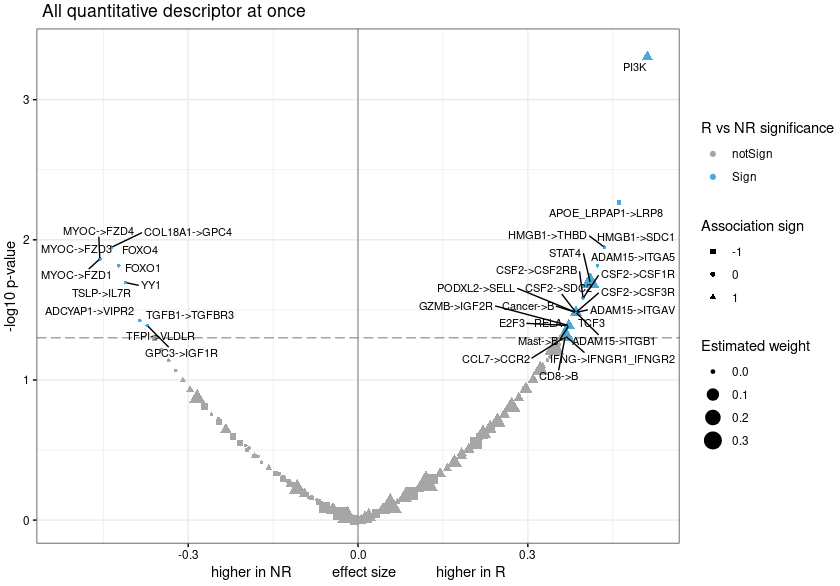
\includegraphics[width=0.95\linewidth,]{easierFinal} \caption{Comparison of genomic features distinguishing patients non-responsive and responsive to immune checkpoint blockade.}\label{fig:easfin}
\end{figure}

This display encapsulates a) the capacity of measurements of
genomic elements to discriminate patients who respond
to ICB for bladder cancer (position of labeled
item on x axis), b) the direction of association of
element activity with immune response (shape of glyph) and c) the
relative magnitudes of weights (size of glyph) estimated for features in
initial model fitting.

The design of this package is noteworthy in its approach
to information hiding. Parameters estimated in machine
learning of tissue-specific relations between quantitative
descriptors of the tumor microenvironment and hallmarks
of immune response are stored in ExperimentHub.

\begin{Shaded}
\begin{Highlighting}[]
\KeywordTok{library}\NormalTok{(easierData)}
\KeywordTok{list\_easierData}\NormalTok{()}
\CommentTok{\#\#     eh\_id                          title}
\CommentTok{\#\# 1  EH6677 Mariathasan2018\_PDL1\_treatment}
\CommentTok{\#\# 2  EH6678                     opt\_models}
\CommentTok{\#\# 3  EH6679               opt\_xtrain\_stats}
\CommentTok{\#\# 4  EH6680            TCGA\_mean\_pancancer}
\CommentTok{\#\# 5  EH6681              TCGA\_sd\_pancancer}
\CommentTok{\#\# 6  EH6682               cor\_scores\_genes}
\CommentTok{\#\# 7  EH6683             intercell\_networks}
\CommentTok{\#\# 8  EH6684              lr\_frequency\_TCGA}
\CommentTok{\#\# 9  EH6685                  group\_lrpairs}
\CommentTok{\#\# 10 EH6686                HGNC\_annotation}
\CommentTok{\#\# 11 EH6687         scores\_signature\_genes}
\end{Highlighting}
\end{Shaded}

The structure of the stored model weights resource can
be sketched by probing list elements.

\begin{Shaded}
\begin{Highlighting}[]
\NormalTok{mw =}\StringTok{ }\NormalTok{eh[[}\StringTok{"EH6678"}\NormalTok{]]}
\CommentTok{\#\# see ?easierData and browseVignettes(\textquotesingle{}easierData\textquotesingle{}) for documentation}
\CommentTok{\#\# loading from cache}
\KeywordTok{names}\NormalTok{(mw)                          }\CommentTok{\# TCGA tumor types}
\CommentTok{\#\#  [1] "LUAD"  "LUSC"  "BLCA"  "BRCA"  "CESC"  "CRC"   "GBM"   "HNSC"  "KIRC" }
\CommentTok{\#\# [10] "KIRP"  "LIHC"  "OV"    "PAAD"  "PRAD"  "SKCM"  "STAD"  "THCA"  "UCEC" }
\CommentTok{\#\# [19] "NSCLC"}
\KeywordTok{names}\NormalTok{(mw[[}\StringTok{"LUAD"}\NormalTok{]])                }\CommentTok{\# TME descriptors}
\CommentTok{\#\# [1] "pathways"    "immunecells" "tfs"         "lrpairs"     "ccpairs"}
\KeywordTok{rownames}\NormalTok{(mw[[}\StringTok{"LUAD"}\NormalTok{]]}\OperatorTok{$}\NormalTok{pathways}\OperatorTok{$}\NormalTok{CYT) }\CommentTok{\# predict cytolytic activity}
\CommentTok{\#\#  [1] "(Intercept)" "Androgen"    "EGFR"        "Estrogen"    "Hypoxia"    }
\CommentTok{\#\#  [6] "JAK{-}STAT"    "MAPK"        "NFkB"        "p53"         "PI3K"       }
\CommentTok{\#\# [11] "TGFb"        "TNFa"        "Trail"       "VEGF"        "WNT"}
                                    \CommentTok{\# using pathway activity}
\end{Highlighting}
\end{Shaded}

The vignette of the easier package steps through phases,
using these tumor-type-specific weights to compute patient-specific measures
of transcription factor activity or cell-cell interaction on the basis of bulk
RNA-seq (units are transcripts per million), and a patient-specific
measure of pathway activity using raw RNA-seq counts. These metrics
may be of interest in their own right for applications other than
establishing predictions of response to ICB.

Appendix \ref{app3} provides the names and versions of all packages
used to produce this analysis.

\subsection{Representing and visualizing a spatial transcriptomics experiment}\label{representing-and-visualizing-a-spatial-transcriptomics-experiment}

\begin{Shaded}
\begin{Highlighting}[]
\KeywordTok{library}\NormalTok{(SpatialFeatureExperiment)}
\KeywordTok{library}\NormalTok{(SFEData)}
\NormalTok{jbr =}\StringTok{ }\KeywordTok{JanesickBreastData}\NormalTok{(}\StringTok{"rep1"}\NormalTok{)}
\NormalTok{jbr}
\CommentTok{\#\# class: SpatialFeatureExperiment }
\CommentTok{\#\# dim: 541 167782 }
\CommentTok{\#\# metadata(1): Samples}
\CommentTok{\#\# assays(1): counts}
\CommentTok{\#\# rownames(541): ABCC11 ACTA2 ... BLANK\_0497 BLANK\_0499}
\CommentTok{\#\# rowData names(6): ID Symbol ... vars cv2}
\CommentTok{\#\# colnames: NULL}
\CommentTok{\#\# colData names(10): Sample Barcode ... nCounts nGenes}
\CommentTok{\#\# reducedDimNames(0):}
\CommentTok{\#\# mainExpName: NULL}
\CommentTok{\#\# altExpNames(0):}
\CommentTok{\#\# spatialCoords names(2) : x\_centroid y\_centroid}
\CommentTok{\#\# imgData names(1): sample\_id}
\CommentTok{\#\# }
\CommentTok{\#\# unit:}
\CommentTok{\#\# Geometries:}
\CommentTok{\#\# colGeometries: centroids (POINT), cellSeg (POLYGON), nucSeg (GEOMETRY) }
\CommentTok{\#\# }
\CommentTok{\#\# Graphs:}
\CommentTok{\#\# sample01:}
\end{Highlighting}
\end{Shaded}

The expression values have strongly skewed distributions.
For exploratory visualization we log-transform.

\begin{Shaded}
\begin{Highlighting}[]
\NormalTok{lfasn=}\KeywordTok{log}\NormalTok{(}\KeywordTok{as.numeric}\NormalTok{(}\KeywordTok{assay}\NormalTok{(jbr[}\StringTok{"FASN"}\NormalTok{,]))}\OperatorTok{+}\DecValTok{1}\NormalTok{)}
\NormalTok{lpostn=}\KeywordTok{log}\NormalTok{(}\KeywordTok{as.numeric}\NormalTok{(}\KeywordTok{assay}\NormalTok{(jbr[}\StringTok{"POSTN"}\NormalTok{,]))}\OperatorTok{+}\DecValTok{1}\NormalTok{)}
\end{Highlighting}
\end{Shaded}

Figure \ref{fig:dospat}

\begin{Shaded}
\begin{Highlighting}[]
\NormalTok{strom =}\StringTok{ }\KeywordTok{ggplot}\NormalTok{(}\KeywordTok{colGeometries}\NormalTok{(jbr)}\OperatorTok{$}\NormalTok{centroids, }\KeywordTok{aes}\NormalTok{(}\DataTypeTok{colour=}\NormalTok{lpostn)) }\OperatorTok{+}
\StringTok{  }\KeywordTok{geom\_sf}\NormalTok{(}\DataTypeTok{size=}\NormalTok{.}\DecValTok{01}\NormalTok{) }\OperatorTok{+}\StringTok{ }\KeywordTok{scale\_color\_viridis\_c}\NormalTok{() }\OperatorTok{+}\StringTok{ }\KeywordTok{ggtitle}\NormalTok{(}\StringTok{"POSTN, stromal"}\NormalTok{)}
\NormalTok{fasn =}\StringTok{ }\KeywordTok{ggplot}\NormalTok{(}\KeywordTok{colGeometries}\NormalTok{(jbr)}\OperatorTok{$}\NormalTok{centroids, }\KeywordTok{aes}\NormalTok{(}\DataTypeTok{colour=}\NormalTok{lfasn)) }\OperatorTok{+}
\StringTok{  }\KeywordTok{geom\_sf}\NormalTok{(}\DataTypeTok{size=}\NormalTok{.}\DecValTok{01}\NormalTok{) }\OperatorTok{+}\StringTok{ }\KeywordTok{scale\_color\_viridis\_c}\NormalTok{() }\OperatorTok{+}\StringTok{ }\KeywordTok{ggtitle}\NormalTok{(}\StringTok{"FASN, invasive"}\NormalTok{)}
\KeywordTok{library}\NormalTok{(gridExtra)}
\KeywordTok{grid.arrange}\NormalTok{(strom, fasn, }\DataTypeTok{ncol=}\DecValTok{2}\NormalTok{)}
\end{Highlighting}
\end{Shaded}

\begin{figure}
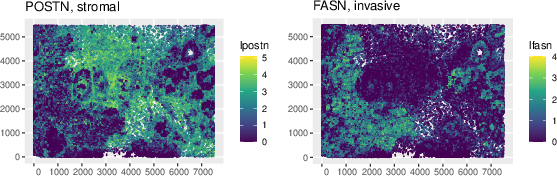
\includegraphics[width=1\linewidth,]{bioccb_files/figure-latex/dospat-1} \caption{Informal rendering of data from Visium studies of breast cancer described in Janesick et al. 2023.}\label{fig:dospat}
\end{figure}

